%%%%%%%%%%%%%%% Updated by MR March 2007 %%%%%%%%%%%%%%%%
\documentclass[12pt]{beamer}
\usetheme{Boadilla}

\newcommand{\al}{$<$}
\newcommand{\ar}{$>$}

\usepackage{listings}
\usepackage{graphicx}
\usepackage{wrapfig}
\graphicspath{ {./graphics/} }

\usepackage{minted}
%\usemintedstyle{colorful}
\setmintedinline{breaklines}

\newcommand{\textinline}{\mintinline{text}}
\newcommand{\cinline}{\mintinline{CGatwick}}
\newcommand{\camlinline}{\mintinline{OCaml}}

\title{Compiling OCaml to WebAssembly}
\author{Paul Durbaba}
\date{10 February 2020}

\begin{document}
	\begin{frame}
		\titlepage
	\end{frame}

	\begin{frame}[fragile]
		\frametitle{Project Idea}
		\begin{itemize}
			\item Compile OCaml to WebAssembly
			\item Implement own type-checker, IR and code generator
			\item WebAssembly: Binary Instruction format for the web
				\begin{itemize}
					\item Stack based, variables, int/float types only, validated when loaded
				\end{itemize}
		\end{itemize}

		\begin{center}
		\begin{minted}[fontsize=\scriptsize]{LISP}
(func $call_closure (export "call_closure")
  (param $closure i32)
  (param $arg i32)
  (result i32)
  
  local.get $closure
  local.get $arg
  local.get $closure
  i32.load offset=0
  call_indirect (param i32 i32) (result i32)
)
		\end{minted}
		\end{center}
	\end{frame}

	\begin{frame}
		\frametitle{What I've Achieved}
		\begin{columns}
			\column{0.5\linewidth}
			\begin{itemize}
				\item Type checker ($\approx$1200 loc) implements Hindley-Milner type inference
				\item Closure conversion ($\approx$250 loc) gives us top level functions
				\item IR Transformation ($\approx$1200 loc) originally structured and stack-based for WebAssembly, now linear n-address code for optimisation
				
			\end{itemize}
			
			\column{0.4\linewidth}
			\begin{center}
				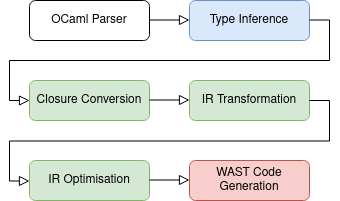
\includegraphics[width=\linewidth]{otwa-stages}
			\end{center}
		\end{columns}
	\end{frame}

	\begin{frame}[fragile]
		\frametitle{What I've Achieved - Continued}
		\begin{columns}
			\column{0.6\linewidth}
			\begin{itemize}
				\item Analysis + Optimisation ($\approx$ 300 loc) mostly analysis so far, only optimisation implemented is copy propagation
				\item Code Generation ($\approx$ 500 loc) outputs WebAssembly
				\item End to End Tester ($\approx$ 250 loc) compiles samples, executes them, and inspects their global values. Support for benchmarking vs OCaml Interpreter only so far.
			\end{itemize}
			\column{0.4\linewidth}
			\begin{center}
				\begin{minted}[fontsize=\scriptsize]{LISP}
local.get $temp0
local.get $n
i32.store offset=4
local.get $temp_0
local.set $add1
local.get $add1
local.set $temp_1
local.get $temp_1
local.get $add1
local.set $temp_2
local.get $temp_2
local.get $add1
local.set $temp_3
local.get $temp_3
local.get $n
local.get $temp_3
i32.load offset=0
				\end{minted}
			\end{center}
			temp\_0 = add1 = temp\_1 = temp\_2 = temp\_3
		\end{columns}
	\end{frame}

	\begin{frame}[fragile]
		\frametitle{What's Next}
		\begin{columns}
			\column{0.8\linewidth}
			\begin{itemize}
				\item Evaluation benchmarks
				\item Negative tests and error messages
				\item More optimisations (guided by the benchmarks)
				\item Strings, records, more syntax support
				\item Garbage collection?
				\item Exceptions?
			\end{itemize}
			\column{0.2\linewidth}
		\end{columns}
		
	\end{frame}
	
\end{document}
